\subsection{简介}
按照官方文档的说明,需要在 trans.c 中写入一个优化的矩阵转置函数。
尽可能地降低不命中率。
使用命令:$./test-trans -M <rol> -N <col>$可以查看这一转置函数的不命中数。
生成的 trace.fi 文件还可以利用 PART A 写的缓存模拟器检查命中情况。

\begin{figure} [H]
    \centering
    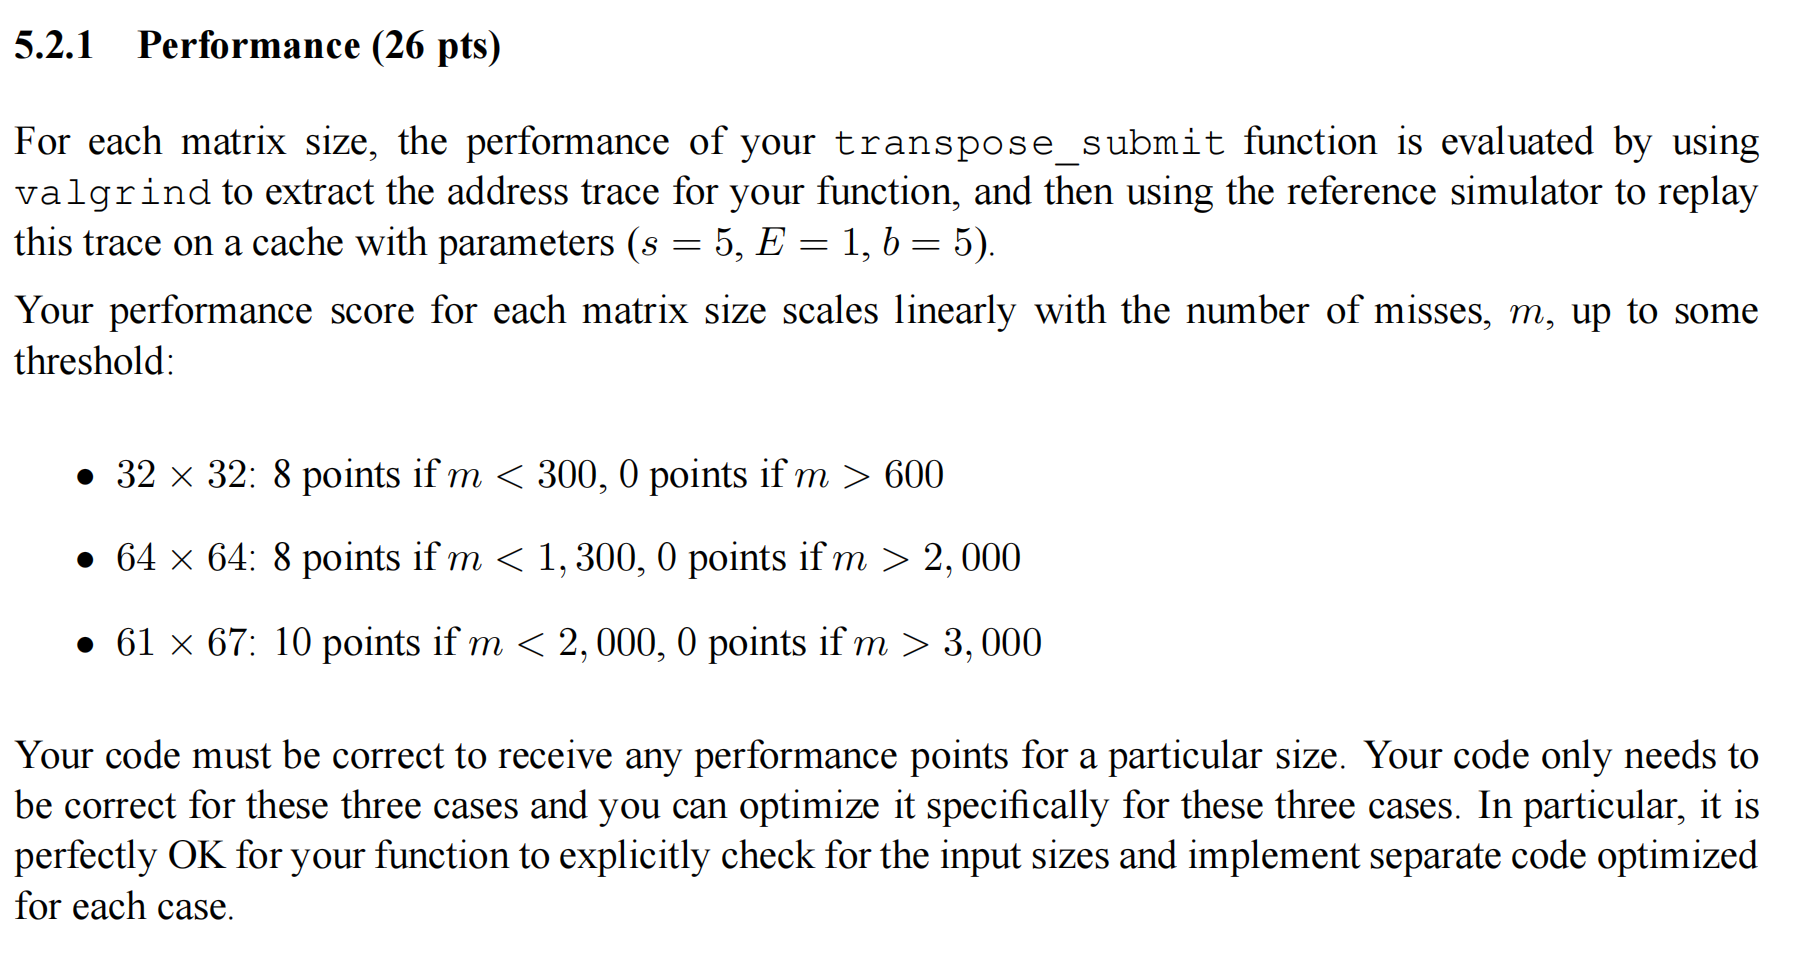
\includegraphics[width=0.52\textwidth]{PartBIntro.png}
    \caption{官方文档简介}
\end{figure}

\subsection{实验内容}
\subsubsection{Part B.1:$ 32 \times 32 $ 矩阵转置}
我们研究最简单的一个矩阵转置函数:
\begin{lstlisting}[language = C,title= Matrix Transpose]
int temp; A[32][32], B[32][32];
for (int i = 0; i < N; i++) {
    for (int j = 0; j < M; j++) {
        tmp = A[i][j];
        B[j][i] = temp;
    }
}
\end{lstlisting}

这是最简单的矩阵转置函数,它具有超过$ 1000 $ 的 $ Miss $数量。
我们可以通过优化这个函数来减少 $ Miss $ 数量。

所以可以利用矩阵分块的思想。每一行数组都可以被存入 4 个缓存行中,
一共有 32 个缓存行,所以每过 8 行就会出现一次和前面相同的组索引,
发生 $ miss $ 和 $ eviction $。所以考虑将 $ 32 \times 32 $ 的矩阵分成$ 16 $个 $8 \times 8 $的矩阵,
每一次都将一行的$ 8 $个 $ int $分别存储进 $t1 - t4$。
即,将矩阵划分成如下结构:

\begin{table}[h!]
    \centering
    \begin{tabular}{|c|c|c|c|}
        \hline
        1 & 2  & 3  & 4  \\
        \hline
        5 & 6  & 7  & 8  \\
        \hline
        9 & 10 & 11 & 12 \\
        \hline
    \end{tabular}
    \caption{Cache Struct (其中每一个小块都是 $ 8 \times 8 $)}
\end{table}

\begin{lstlisting}[language = C,title= Matrix Transpose]
/* 
* transpose_submit - This is the solution transpose function that you
*     will be graded on for Part B of the assignment. Do not change
*     the description string "Transpose submission", as the driver
*     searches for that string to identify the transpose function to
*     be graded. 
*/
char transpose_submit_desc[] = "Transpose submission";
void transpose_submit(int M, int N, int A[N][M], int B[M][N])
{
    if (N == 32 && M == 32)
    {
        int i, j, k;
        int t1, t2, t3, t4, t5, t6, t7, t8;
        for (i = 0; i < 32; i += 8)
        {
            for (j = 0; j < 32; j += 8)
            {
                for (k = 0; k < 8; k++)
                {
                    t1 = A[i + k][j];
                    t2 = A[i + k][j + 1];
                    t3 = A[i + k][j + 2];
                    t4 = A[i + k][j + 3];
                    t5 = A[i + k][j + 4];
                    t6 = A[i + k][j + 5];
                    t7 = A[i + k][j + 6];
                    t8 = A[i + k][j + 7];
                    B[j][i + k] = t1;
                    B[j + 1][i + k] = t2;
                    B[j + 2][i + k] = t3;
                    B[j + 3][i + k] = t4;
                    B[j + 4][i + k] = t5;
                    B[j + 5][i + k] = t6;
                    B[j + 6][i + k] = t7;
                    B[j + 7][i + k] = t8;
                }
            }
        }
    }
}
\end{lstlisting}

实验结果如下所示:
\begin{figure} [H]
    \centering
    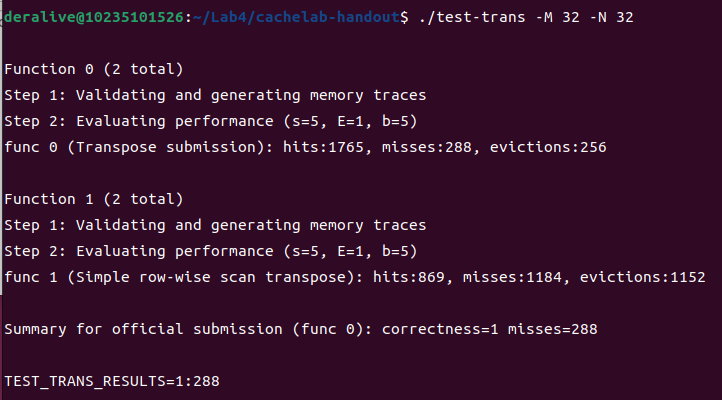
\includegraphics[width=0.52\textwidth]{PartB1.png}
    \caption{Part B.1 结果}
\end{figure}

\subsubsection{Part B.2:$ 64 \times 64 $ 矩阵转置}
大小变成了  $64 \times 64$ ,每过 $4$ 行就会出现一次冲突的情况。

所以可以先分成$ 8 \times 8 $ 的块,然后再把 $8 \times 8$ 的块分成 $4$ 个 $4 \times 4 $的块。

我们这里需要优化的不是程序运行的时间,而是cache的命中率。
具体是每一个$8 \times 8 $ 块中,分别移动$4 \times 4$ 的块,这样可以减少冲突。

\begin{itemize}
    \item 将 $ 8 \times 8  fence $分成 $ 4 \times 4 $ 的 fence, 再将角块分为 $ A、 B 、C、D$;
    \item 将$A $区的第一行缓存到$A' $和 $C'$ 的第一列
    \item 全部存到$ A' $和 $C'$ 后,再将C' 的第一列存到$ Temp1 \& Temp2 \& Temp3 \& Temp4 $变量当中
    \item 手动交换$C'$ 区 和 $B'$ 区的各个数值
\end{itemize}

\begin{figure} [H]
    \centering
    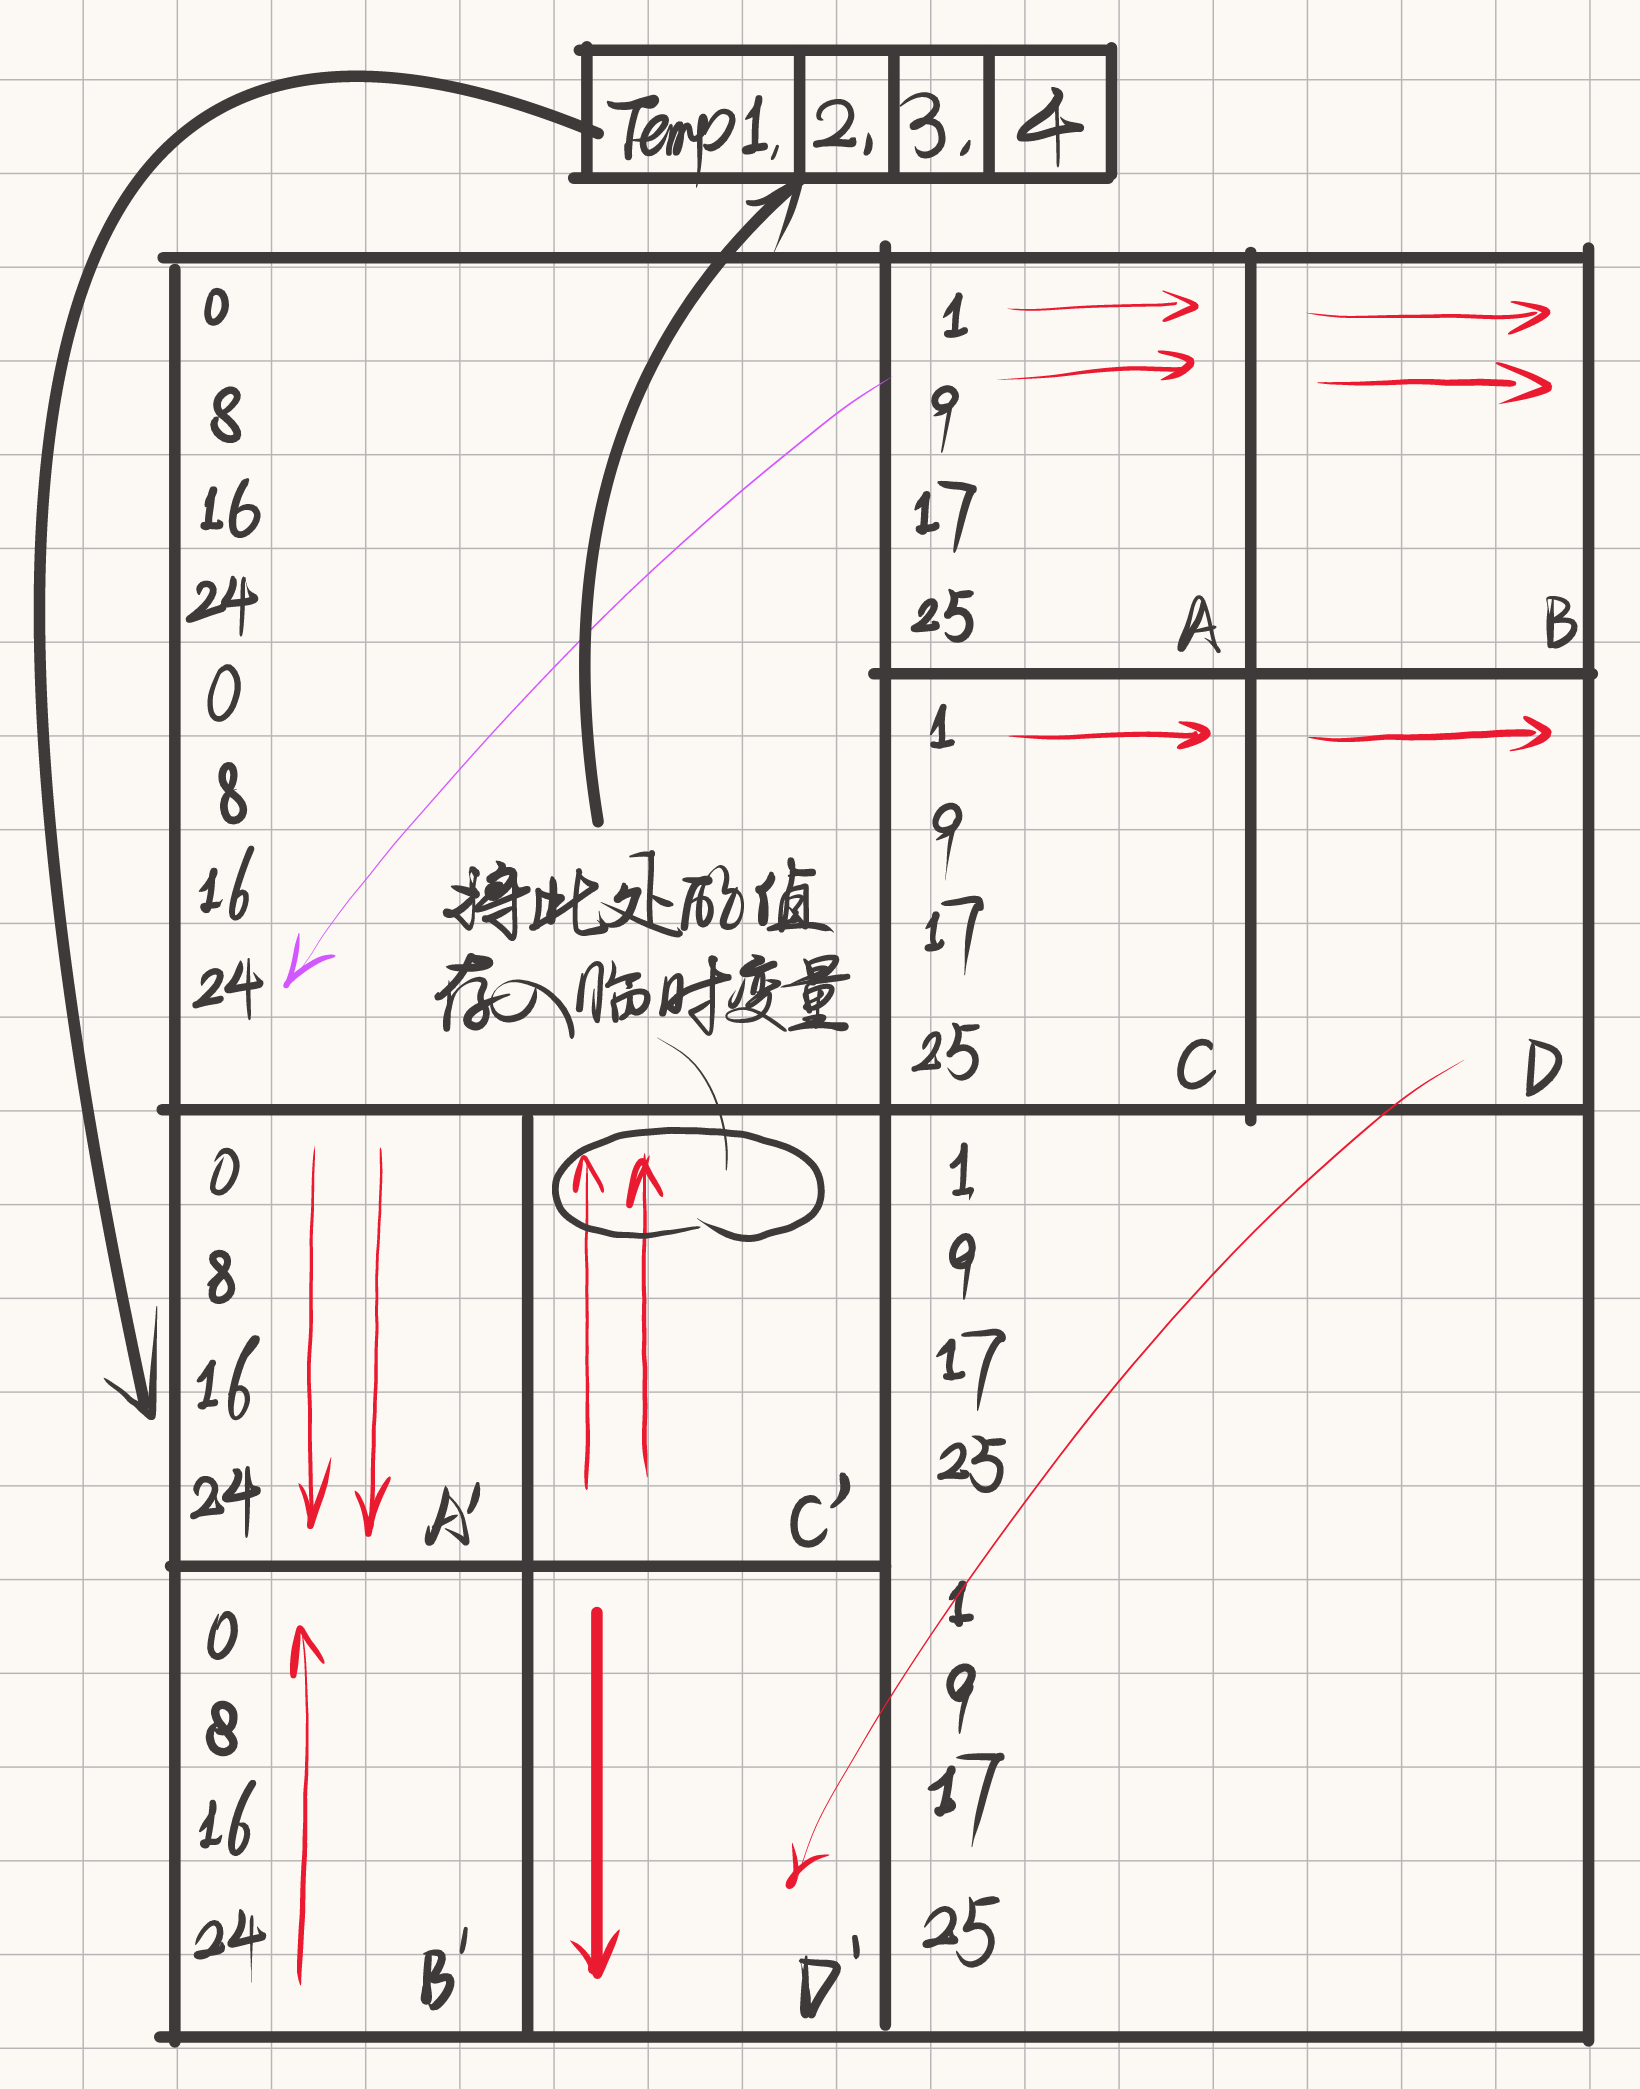
\includegraphics[width=0.38\textwidth]{Analy.png}
    \caption{Analysis Process}
\end{figure}


\begin{lstlisting}[language = C,title= Matrix Transpose]
else if (N == 64 && M == 64)
{
    int t0, t1, t2, t3, t4, t5, t6, t7;
    for (int i = 0; i < N; i += 8)
    {
        for (int j = 0; j < M; j += 8)
        {
            for (int k = i; k < i + 4; k++)
            {
                t0 = A[k][j];
                t1 = A[k][j + 1];
                t2 = A[k][j + 2];
                t3 = A[k][j + 3];
                t4 = A[k][j + 4];
                t5 = A[k][j + 5];
                t6 = A[k][j + 6];
                t7 = A[k][j + 7];
                B[j][k] = t0;
                B[j + 1][k] = t1;
                B[j + 2][k] = t2;
                B[j + 3][k] = t3;
                B[j + 0][k + 4] = t7;
                B[j + 1][k + 4] = t6;
                B[j + 2][k + 4] = t5;
                B[j + 3][k + 4] = t4;
            }
            for (int h = 0; h < 4; h++)
            {
                t0 = A[i + 4][j + 3 - h];
                t1 = A[i + 5][j + 3 - h];
                t2 = A[i + 6][j + 3 - h];
                t3 = A[i + 7][j + 3 - h];
                t4 = A[i + 4][j + 4 + h];
                t5 = A[i + 5][j + 4 + h];
                t6 = A[i + 6][j + 4 + h];
                t7 = A[i + 7][j + 4 + h];
                B[j + 4 + h][i + 0] = B[j + 3 - h][i + 4];
                B[j + 4 + h][i + 1] = B[j + 3 - h][i + 5];
                B[j + 4 + h][i + 2] = B[j + 3 - h][i + 6];
                B[j + 4 + h][i + 3] = B[j + 3 - h][i + 7];
                B[j + 3 - h][i + 4] = t0;
                B[j + 3 - h][i + 5] = t1;
                B[j + 3 - h][i + 6] = t2;
                B[j + 3 - h][i + 7] = t3;
                B[j + 4 + h][i + 4] = t4;
                B[j + 4 + h][i + 5] = t5;
                B[j + 4 + h][i + 6] = t6;
                B[j + 4 + h][i + 7] = t7;
            }
        }
    }
}
\end{lstlisting}

实验结果如下所示:

\begin{figure} [H]
    \centering
    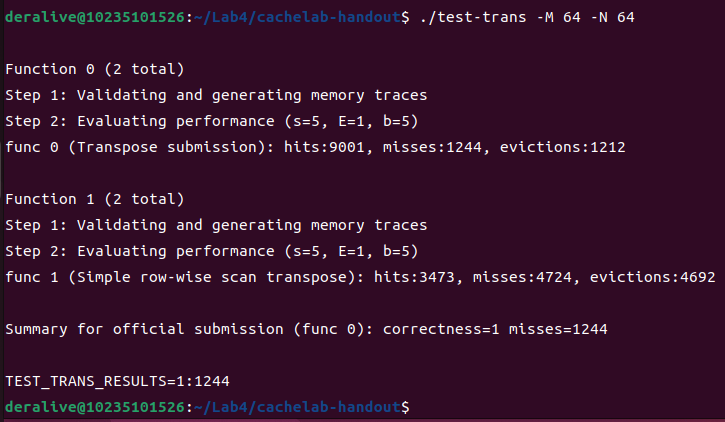
\includegraphics[width=0.52\textwidth]{PartB2.png}
    \caption{Part B.2 结果}
\end{figure}

\subsubsection{Part B.3:$ 61 \times 67 $ 矩阵转置}
这里的矩阵大小是 $61 \times 67$ ,这个矩阵的大小是一个奇数,所以不能被整除。
而且也不是 $ 8 $ 的倍数,所以在行与行之间没有特别明显的冲突不命中的关系。
可以尝试用分块矩阵的方式优化。经过尝试 $ 8 \times 8 $ 的分块和 $ 16 \times 16 $的分块后,
发现使用 $16 \times 16 $的分块方式可以将 $Miss$ 数降低到 $ 2000 $以下。

代码如下所示:
\begin{lstlisting}[language = C,title= Matrix Transpose]
else {
    int i, j, k, h;
    for (i = 0; i < N; i += 16) {
        for (j = 0; j < M; j += 16) {
            for (k = i; k < i + 16 && k < N; k++) {
                for (h = j; h < j + 16 && h < M; h++) {
                    B[h][k] = A[k][h];
                }
            }
        }
    }
}
\end{lstlisting}

实验结果如下所示:

\begin{figure} [H]
    \centering
    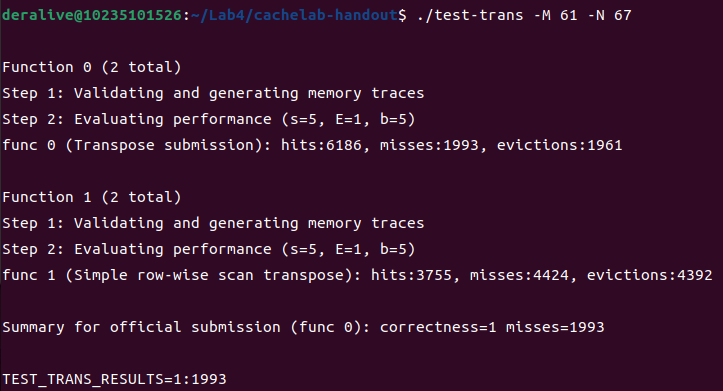
\includegraphics[width=0.52\textwidth]{PartF.png}
    \caption{Part B.3 结果}
\end{figure}





